\section{\gls{dbscan}}
\label{sec:dbscan}

\subsection{Overview}

\begin{figure}[htbp]
    \centering
    \begin{subfigure}{\textwidth}
    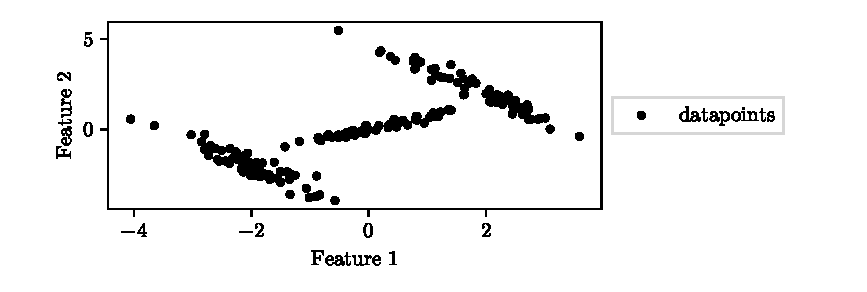
\includegraphics[width=\textwidth]{images/DBSCAN/Figure_1.pdf}
    \caption{training data}
    \label{fig:dbscandata}
    \end{subfigure}
    \begin{subfigure}{\textwidth}
    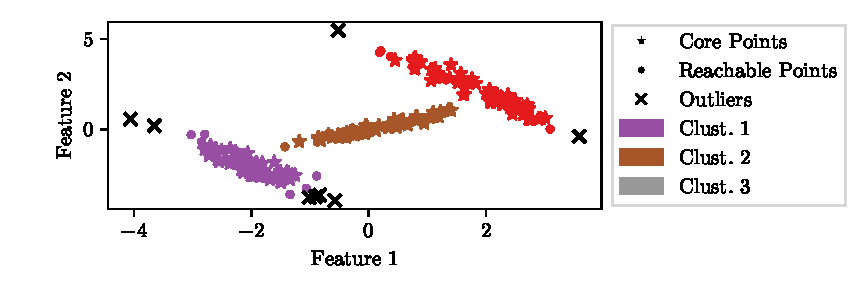
\includegraphics[width=\textwidth]{images/DBSCAN/Figure_2.pdf}
    \caption{training result}
    \label{fig:dbscanresult}
    \end{subfigure}
    \caption{\gls{dbscan} clustering}
    \label{fig:dbscan}
\end{figure}

\begin{figure}
    \centering
    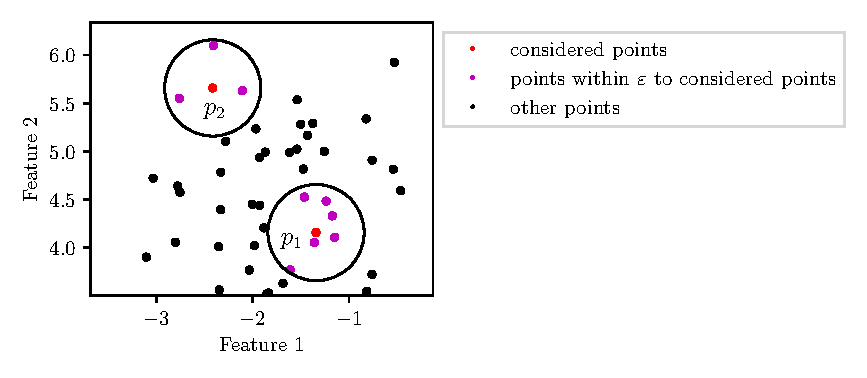
\includegraphics[width=\textwidth]{images/DBSCAN/Figure_3.pdf}
    \caption{Example of core and border points}
    \label{fig:dbscanparams}
\end{figure}

Looking at \autoref{fig:dbscandata} we can see that the data are clearly divided into $3$ clusters, but a simple K-means will fail to cluster correctly the data because the clusters are very stretched. 
But how do we humans see that there are $3$ clusters? We instinctively look at the density of the points, and we can see that there are $3$ areas with a high density of points, and the rest of the space is empty. \gls{dbscan} is a clustering algorithm that tries to mimic this behaviour.

\gls{dbscan} is a density-based clustering designed by Martin Ester, Hans-Peter Kriegel, Jörg Sander and Xiaowei Xu \cite{dbscan}. The algorithm is based on the definition of what a  \emph{core point} is, and what a \emph{density-reachable} point is.


The algorithm inputs are:
\begin{itemize}
    \item $D$: the dataset
    \item $\varepsilon$: the radius of the neighbourhood
    \item $MinPts$: the minimum number of points to form a cluster
\end{itemize}

The basic idea is that if a point has a sufficient number of other points ($MinPts$) in its neighbourhood of radius $\varepsilon$, then it is a \emph{core point}. Chosen a core point, all the other core points in its neighbourhood are assigned to the same cluster, and the process is repeated for all the core points in the neighbourhood of the just assigned ones and so on. At a certain point there will be a cluster of core points that are not near any other core point, when this happens the idea is to include in the cluster also the points that are not core points but are in the neighbourhood of the core points of the cluster. 

To better visualize the process, \autoref{fig:dbscanparams} shows some data points. Let's assume $MinPts = 5$ The point $p_1$ is a core point because, in its neighbourhood of radius $\varepsilon$, there are $7>MinPts$ points. The point $p_2$ is not a core point because in its neighbourhood there are only $3<MinPts$ points. even if it is not a core point, it may be assigned to a cluster, depending on if there is a core point in its neighbourhood. If a point is not a core point and there is not a core point in its neighbourhood, then it is a noise point and it is not assigned to any cluster. 

Some of the definitions presented in \cite{dbscan} can be resumed for our purpose as follows:
\begin{itemize}
    \item $N_\varepsilon(p) = {q\in D : \norm{\gls{sym:dist}\le \varepsilon}}$ is the set of points in the $\varepsilon$-neighbourhood of $p$;
    \item a point $p$ is a \emph{core point} if there are at least $MinPts$ points in the $\varepsilon$-neighbourhood of $p$;
    \item a point $p$ is \emph{directly density-reachable} from $q$ if $p$ is in the $\varepsilon$-neighbourhood of $q$ and $q$ is a core point;
    \item a point $p$ is \emph{density-reachable} from $q$ if there is a chain of points $p_1, \dots, p_n$ such that $p_1 = q$ and $p_n = p$ and $p_{i+1}$ is directly density-reachable from $p_i$;
    \item a point $p$ is \emph{density-connected} to $q$ if there is a point $o$ such that both $p$ and $q$ are density-reachable from $o$;
\end{itemize}

In the paper \cite{dbscan} the authors propose a detailed pseudocode of the algorithm, \autoref{alg:dbscan} is a more abstract version of it.
\begin{algorithm}
    \caption{Train \gls{dbscan}}
  \label{alg:dbscan}
  \begin{algorithmic}[1]
    \Procedure{\gls{dbscan}}{$D, \varepsilon, MinPts$}
    \For {$p \in D$}
        \If {$\abs{N_\varepsilon(p)} \ge MinPts$}
            \State mark $p$ as a core point
        \EndIf
    \EndFor
    \State $i \gets 0$ \Comment{cluster index}
    \While{there are unassigned points}
        \State $\gls{glo:clust}_i \gets \emptyset $
        \State choose an unassigned point $p$
        \State $\gls{glo:clust}_i \gets \gls{glo:clust}_i \cup p $ \Comment{add $p$ to the cluster}
        \For {$ q \in $ all reachable points from $p$}
            \LineComment{all density-reachable points from $p$ are added to the cluster}
            \State $\gls{glo:clust}_i \gets \gls{glo:clust}_i \cup q  $ \Comment{add $q$ to the cluster}
        \EndFor
        \If {there are no unassigned core points}
            \State drop all unassigned points from $D$ \Comment{they are noise}
            \EndIf
        \State $i \gets i + 1$
    \EndWhile
    \EndProcedure
  \end{algorithmic}
\end{algorithm}

\subsection{Choosing the parameters}
Running the algorithm implemented in the \texttt{sklearn} library on the dataset of \autoref{fig:dbscandata} with $\varepsilon = 0.78$ and $MinPts = 10$ we obtain the result of \autoref{fig:dbscanresult}. The algorithm correctly identifies the $3$ clusters, also the noise points number is affected by the choice of $\varepsilon$ and $MinPts$.

Note that the \gls{dbscan} is able to identify clusters with arbitrary shapes, even if they are not convex and are not \gls{glo:lin-sep}. This is a big advantage over the K-means, which is not able to identify clusters with arbitrary shapes.


\begin{figure}
    \centering
    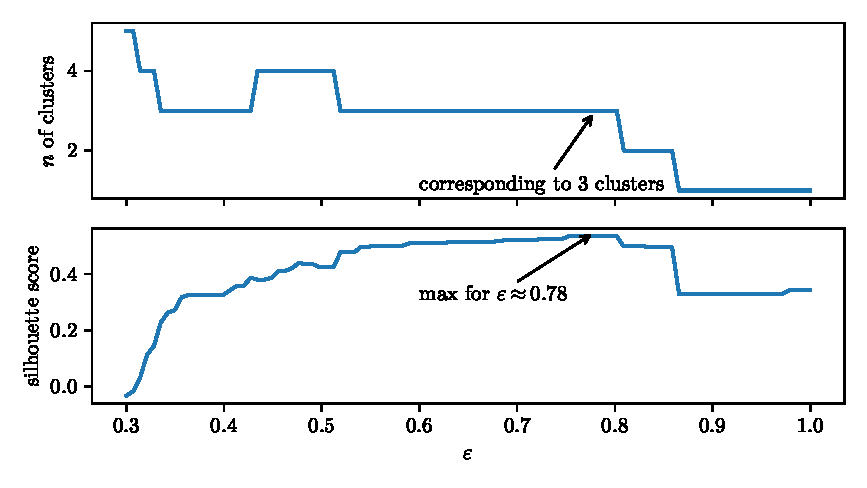
\includegraphics{images/DBSCAN/Figure_4.pdf}
    \caption{Silhouette score for different values of $\varepsilon$}
    \label{fig:dbscansilhouette}
\end{figure}

Even being the \gls{dbscan} an unsupervised algorithm, it has some parameters that need to be set by the user.
The first parameter is $\varepsilon$, the radius of the neighbourhood. This gives a measure of the density we expect from the clusters. As seen for the K-means in \autoref{sec:kmeans}, we can try to find the best $\varepsilon$ by using the silhouette score.

Let's plot the silhouette score for different values of $\varepsilon$ to confirm that using $\varepsilon = 0.78$ is a good choice. In the \autoref{fig:dbscansilhouette} are shown the results that link the best $\varepsilon$ value to $3$ cluster being generated.

\subsection{Evaluation of a new instance}
\label{sec:dbscan_eval}
Assume now that the training of the \gls{dbscan} is complete, and a new \gls{glo:snap} $\gls{sym:snap}_n$ is generated from the sensor data. How can we evaluate if the new snapshot is novel or not?
The \gls{dbscan} algorithm is not able to predict the cluster of a new instance. However, the task of this project is novelty detection, not classification.
To do that, as has been done for the K-means, a metric linked to how novel a new snapshot is developed. 

The idea used previously to compute the distance to a centroid and normalizing it by the radius of the cluster is not applicable here, because the \gls{dbscan} do not use centroids to define clusters. A naive idea for our purpose is to compute the distance of the new snapshot from the closest snapshot in the training dataset.
If the distance is greater than a threshold, then the new snapshot is considered novel.

And now the question: if we use the distance of a new $\gls{sym:snap}_n$ from the closest $\gls{sym:snap}_i$ in the training dataset (spanning the whole dataset to compute it) why did we train a model in the first place? Wouldn't it be simpler to just apply this metric to the training dataset without clustering it? As far as concerns scope of this thesis, performing the clustering first has two main advantages:
\begin{itemize}
    \item $\varepsilon$ has been chosen running the \gls{dbscan}, so nobody had to guess it. This is a big advantage because the choice of $\varepsilon$ would be very difficult to do with limited knowledge of the monitored system. Normalizing the computed distance by $\varepsilon$ we can obtain a measure of how novel a snapshot is for which we can set a threshold without tuning it on the specific system;
    \item during the training phase, the \gls{dbscan} has discarded the noise points. This improves the quality of the metric because the distance from a noise point is not meaningful.
\end{itemize}

\subsection{Limitations of the algorithm}
The first limitation of \gls{dbscan} is about cluster density: since $\varepsilon$ is fixed, the algorithm is not able to identify clusters with different densities. In this case, it will split low-density clusters into multiple clusters. For our purpose, this is not a problem, because we are interested in novelty detection, so even if a cluster is misidentified as multiple clusters, the new snapshot will be considered novel. To increase the sensitivity of the novelty detection $\varepsilon$ can be decreased, but this will increase the number of noise points.

The other main limitation of \gls{dbscan} is that it has a complexity of roughly $\mathcal{O}(m^2)$, where $m$ is the number of points in the dataset. This means that the algorithm is not scalable to large datasets \citepage{hands-on-geron2022}{281}. There exist improvements to the algorithm that reduce the complexity to $\mathcal{O}(m\log m)$, like the FDBSCAN developed by Bing Liu \cite{dbscanlogm}. The complexity remains linear \gls{wrt} the number of features.
